\documentclass[10pt,a4paper]{article}
\usepackage[utf8]{inputenc}
\usepackage{amsmath}
\usepackage{amsfonts}
\usepackage{amssymb}
\usepackage{graphicx}
\usepackage{tikz}
\usetikzlibrary{shapes}
\usepackage[colorlinks=true, urlcolor=blue, linkcolor=red]{hyperref}
\author{Parker}
\title{Calculating Height from Video}
\begin{document}
\maketitle

The following calculations are an attempt to derive the height and width (of the crown) of a tree from a drone video \textbf{assuming knowledge of the drone's attitude, position, and velocity}. We will model the tree as a cylinder. 

We first consider what the drone sees. Figure \ref{DroneImage} is a possible example of a video frame where $\tau$ represents the placement of the tree. Assuming the camera is not gimballed (a correction we can easily account for later), the center of the box is the $x$-body coordinate, a known direction as the attitude is known. Let $W_P$ and $H_P$ be the number of pixels of the width and height of the frame, respectively. Let $\phi_P$ and $\psi_P$ be the number of pixels along the width and height, respectively, from the center of the frame \textbf{to the center of the tree}, as determined by the bounding box. Let $\beta$ and $\alpha$ be the width and height angles respectively of the frame. Then we can define $\phi = \frac{\beta\phi_P}{W_P}$ and $\psi=\frac{\alpha \psi_P}{H_P}$. Then we can compute the line of sight vector $l$ by applying the rotation matrices to the body $x$-axis: $l = R^{y'}(\psi)R^z(\phi)x_{body}$. 

To find a system of equations which allows us to estimate the height of the cylinder, let us consider a cylinder of height $h_t$ and diameter $w$ and compute $\psi_P$ for a given drone height $h_v$ and distance $d$ to the tree center (we for now assume $d >> h_t, w$). See fig. \ref{DroneDiagram}. Let $\gamma$ be the angle that $d$ makes with the ground (with our assumption we treat the tree center as if it is on the ground). Then the ``height'' of the tree appears to the drone as a combination of its true height and width: 
\begin{equation}
\psi_a = \cos(\gamma)h_t + \sin(\gamma)w = \sqrt{1-\left(\frac{h_v}{d}\right)^2}h_t + \frac{h_v}{d}w
\end{equation} 
To find out how many pixels this occupies on the drone's frame, we consider that at distance $d$, an angle of $\alpha$ covers a height of $d\alpha$. If the total number of height pixels is $H_P$, then we compute
\begin{equation}
\psi_P =\frac{H_P}{d\alpha}\left[\sqrt{1-\left(\frac{h_v}{d}\right)^2}h_t + \frac{h_v}{d}w\right]
\end{equation}
  Suppose that this frame is the first in a sequence, so that we use the label $\psi^{(1)}_P$ and $d^{(1)}$. Also suppose that the drone is flying with a small enough acceleration so that the velocity $v$ is essentially constant over the next few frames. Then we can compute the change in distance $d$ over a time period $t$ to be $(v\cdot l)t$. For short enough $t$ and $2t$, we can compute $d^{(2)}$ and $d^{(3)}$ as $d^{(1)} + (v\cdot l)t$ and $d^{(1)} + 2(v\cdot l)t$, respectively. We therefore have 3 equations and 3 unknowns.
\begin{figure}\label{DroneImage}
\centering
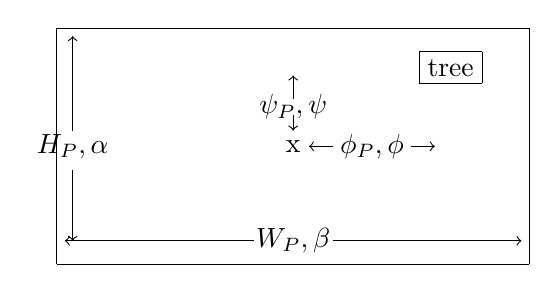
\begin{tikzpicture}
\draw[-] (-3,0) -- (3, 0);
\draw[-] (-3,0) -- (-3, 3);
\draw[-] (-3,3) -- (3, 3);
\draw[-] (3,0) -- (3, 3);

\draw[->] (0.5,0.3) -- (2.9, 0.3);
\draw[->] (-0.5,0.3) -- (-2.9, 0.3);
\node[] at (0,0.3) {$W_P, \beta$};

\draw[<-] (-2.8,0.3) -- (-2.8, 1.2);
\draw[->] (-2.8,1.7) -- (-2.8, 2.9);
\node[] at (-2.8,1.5) {$H_P, \alpha$};

\draw[<-] (0.2,1.5) -- (0.5, 1.5);
\draw[->] (1.5,1.5) -- (1.8, 1.5);
\node[] at (1,1.5) {$\phi_P, \phi$};

\draw[<-] (0,1.7) -- (0, 1.9);
\draw[->] (0,2.1) -- (0, 2.4);
\node[] at (0,2) {$\psi_P, \psi$};

\node[] at (2,2.5) {tree};
\draw[-] (1.6,2.3) -- (2.4, 2.3);
\draw[-] (1.6,2.7) -- (2.4, 2.7);
\draw[-] (1.6,2.3) -- (1.6, 2.7);
\draw[-] (2.4,2.3) -- (2.4, 2.7);

\node[] at (0,1.5) {x};

\end{tikzpicture}
\caption{example video frame}
\end{figure}

\begin{figure}\label{DroneDiagram}
\centering
\begin{tikzpicture}
\draw[-] (-3,0) -- (-3, 3);

\draw[-] (-3, 3) -- (3, 0);
\node[] at (0, 1.7) {d};
\draw[-] (-3,0) -- (3, 0);
\node[] at (-3.2, 1.5) {$h_v$};
\node[] at (-3,3.3) {drone};
\node (A) at (2, 0.5) [cylinder, shape border rotate=90, draw, minimum height=1.5cm, minimum width=0.5cm]{};
\draw [<->] (A.before top) -- (A.after top) node [midway, above, fill=white]{};
\node[] at (1.5,0.5) {$h_t$};
\node[] at (2,1.6) {$w$};
\end{tikzpicture}
\caption{diagram of drone in relation to tree}
\end{figure}


\end{document}